\documentclass[tikz,border=2pt]{standalone}
\usepackage{mathptmx}
\usetikzlibrary{arrows.meta,positioning,fit,calc}
\begin{document}
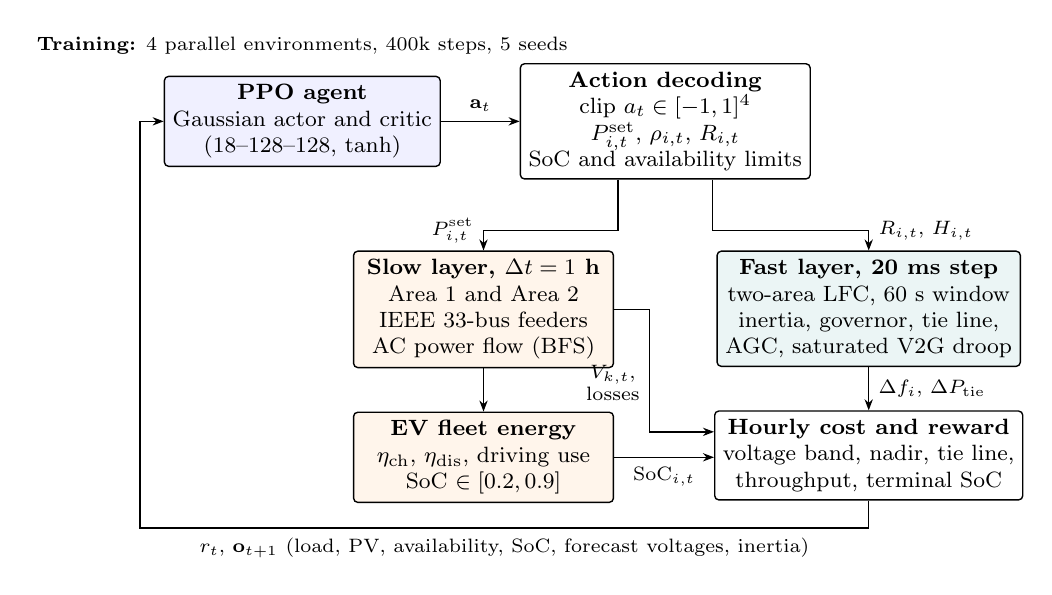
\begin{tikzpicture}[
  font=\footnotesize,
  box/.style={draw, rounded corners=1.5pt, align=center, inner sep=3pt, line width=0.5pt, fill=white},
  agent/.style={box, fill=blue!6},
  slow/.style={box, fill=orange!8},
  fast/.style={box, fill=teal!8},
  arr/.style={-{Stealth[length=4pt]}, line width=0.5pt},
  lbl/.style={font=\scriptsize, align=center}
]
\node[agent, minimum width=3.4cm] (agent) {\textbf{PPO agent}\\Gaussian actor and critic\\(18--128--128, tanh)};
\node[box, right=1.0cm of agent, minimum width=3.6cm] (dec) {\textbf{Action decoding}\\clip $a_t\in[-1,1]^4$\\$P^{\mathrm{set}}_{i,t}$, $\rho_{i,t}$, $R_{i,t}$\\SoC and availability limits};
\draw[arr] (agent) -- node[above, lbl]{$\mathbf{a}_t$} (dec);

\node[slow, below left=0.9cm and -1.2cm of dec, minimum width=3.3cm] (pf) {\textbf{Slow layer, $\Delta t=1$ h}\\Area 1 and Area 2\\IEEE 33-bus feeders\\AC power flow (BFS)};
\node[fast, below right=0.9cm and -1.2cm of dec, minimum width=3.3cm] (lfc) {\textbf{Fast layer, 20 ms step}\\two-area LFC, 60 s window\\inertia, governor, tie line,\\AGC, saturated V2G droop};
\node[slow, below=0.55cm of pf, minimum width=3.3cm] (soc) {\textbf{EV fleet energy}\\$\eta_{\mathrm{ch}}$, $\eta_{\mathrm{dis}}$, driving use\\SoC $\in[0.2,0.9]$};
\draw[arr] (dec.south) ++(-0.6,0) |- ($(pf.north)+(0,0.25)$) -| (pf.north) node[pos=0.0, left, lbl]{$P^{\mathrm{set}}_{i,t}$};
\draw[arr] (dec.south) ++(0.6,0) |- ($(lfc.north)+(0,0.25)$) -| (lfc.north) node[pos=0.0, right, lbl]{$R_{i,t}$, $H_{i,t}$};
\draw[arr] (pf) -- (soc);

\node[box, below=0.55cm of lfc, minimum width=3.3cm] (rew) {\textbf{Hourly cost and reward}\\voltage band, nadir, tie line,\\throughput, terminal SoC};
\draw[arr] (lfc) -- node[right, lbl]{$\Delta f_i$, $\Delta P_{\mathrm{tie}}$} (rew);
\draw[arr] (soc.east) -- node[below, lbl]{SoC$_{i,t}$} (soc.east -| rew.west);
\draw[arr] (pf.east) -- ++(0.45,0) |- node[pos=0.3, left, lbl]{$V_{k,t}$,\\ losses} ($(rew.west)+(0,0.3)$);
\draw[arr] (rew.south) -- ++(0,-0.35) -| node[pos=0.25, below, lbl]{$r_t$, $\mathbf{o}_{t+1}$ (load, PV, availability, SoC, forecast voltages, inertia)} ([xshift=-0.3cm]agent.west) -- (agent.west);
\node[lbl, above=0.15cm of agent] {\textbf{Training:} 4 parallel environments, 400k steps, 5 seeds};
\end{tikzpicture}
\end{document}
